\documentclass[border=8pt]{standalone}
\usepackage{tikz}
\usetikzlibrary{arrows.meta,shapes.geometric,positioning}

\tikzset{
  box/.style={rectangle, rounded corners=3pt, draw=black, line width=0.5pt,
    fill={rgb,255:red,205;green,205;blue,244}, minimum width=2.5cm,
    minimum height=0.95cm, align=center, font=\small},
  db/.style={cylinder, shape border rotate=90, aspect=0.28, draw=black,
    line width=0.5pt, fill={rgb,255:red,200;green,230;blue,201},
    minimum width=1.9cm, minimum height=1.25cm, align=center, font=\small},
  note/.style={font=\itshape\footnotesize, text=black!55, align=center},
  ar/.style={-{Latex[length=2.4mm,width=2mm]}, line width=0.6pt},
  panel/.style={font=\bfseries},
}

\begin{document}
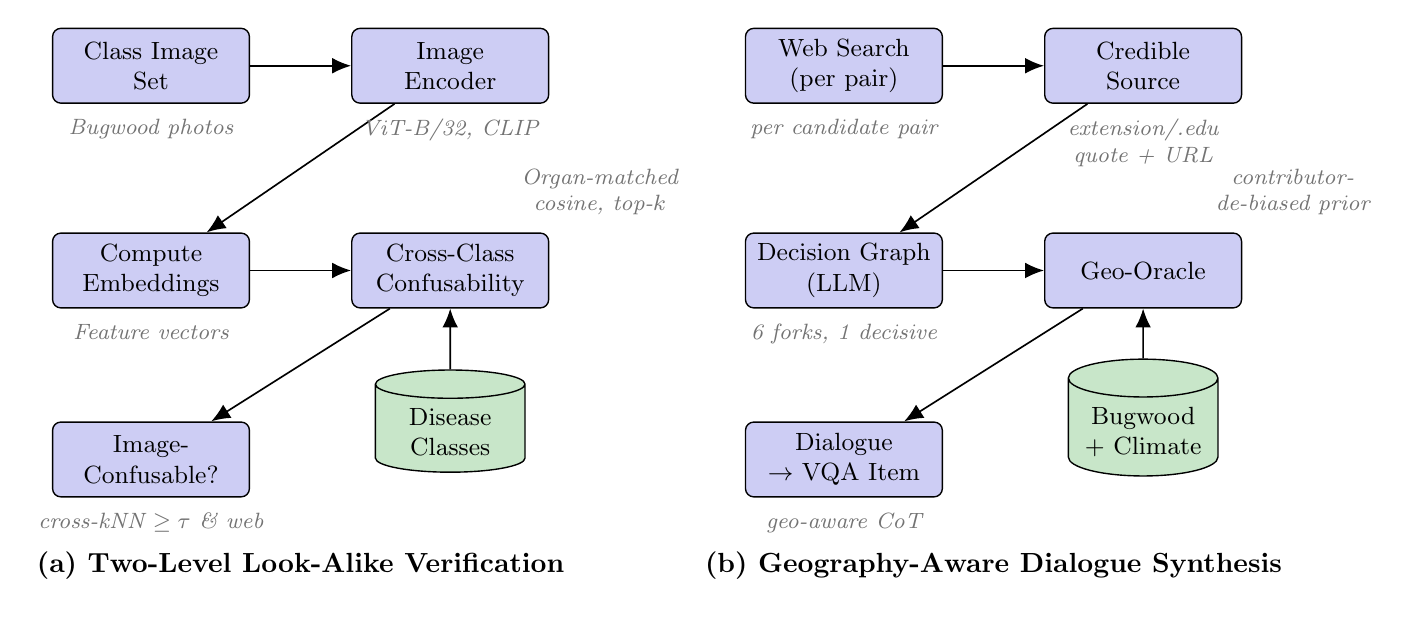
\begin{tikzpicture}[node distance=1cm]

% ===================== PANEL (a) : LOOK-ALIKE VERIFICATION =====================
\begin{scope}[local bounding box=A]
  \node[box] (a1) at (0,6.2)   {Class Image\\Set};
  \node[box] (a2) at (3.8,6.2) {Image\\Encoder};
  \node[box] (a3) at (0,3.6)   {Compute\\Embeddings};
  \node[box] (a4) at (3.8,3.6) {Cross-Class\\Confusability};
  \node[db]  (a5) at (3.8,1.55){Disease\\Classes};
  \node[box] (a6) at (0,1.2)   {Image-\\Confusable?};

  \draw[ar] (a1) -- (a2);
  \draw[ar] (a2) -- (a3);
  \draw[ar] (a3) -- (a4);
  \draw[ar] (a5) -- (a4);
  \draw[ar] (a4) -- (a6);

  \node[note, below=2pt of a1] {Bugwood photos};
  \node[note, below=2pt of a2] {ViT-B/32, CLIP};
  \node[note, below=2pt of a3] {Feature vectors};
  \node[note] at (5.7,4.6) {Organ-matched\\cosine, top-$k$};
  \node[note, below=2pt of a6] {cross-kNN $\geq \tau$ \& web};
\end{scope}

\node[panel] at (1.9,-0.15) {(a) Two-Level Look-Alike Verification};

% ===================== PANEL (b) : DIALOGUE SYNTHESIS =====================
\begin{scope}[xshift=8.8cm, local bounding box=B]
  \node[box] (b1) at (0,6.2)   {Web Search\\(per pair)};
  \node[box] (b2) at (3.8,6.2) {Credible\\Source};
  \node[box] (b3) at (0,3.6)   {Decision Graph\\(LLM)};
  \node[box] (b4) at (3.8,3.6) {Geo-Oracle};
  \node[db]  (b5) at (3.8,1.55){Bugwood\\+ Climate};
  \node[box] (b6) at (0,1.2)   {Dialogue\\$\rightarrow$ VQA Item};

  \draw[ar] (b1) -- (b2);
  \draw[ar] (b2) -- (b3);
  \draw[ar] (b3) -- (b4);
  \draw[ar] (b5) -- (b4);
  \draw[ar] (b4) -- (b6);

  \node[note, below=2pt of b1] {per candidate pair};
  \node[note, below=2pt of b2] {extension/.edu\\quote + URL};
  \node[note, below=2pt of b3] {6 forks, 1 decisive};
  \node[note] at (5.7,4.6) {contributor-\\de-biased prior};
  \node[note, below=2pt of b6] {geo-aware CoT};
\end{scope}

\node[panel] at (10.7,-0.15) {(b) Geography-Aware Dialogue Synthesis};

\end{tikzpicture}
\end{document}
